\section{[Completed] IP Camera}

This project proposes two different methods for near realtime, wireless, cheap video transmission. Keep in mind that the research done by this singular project completely dwarfs every single other project in this document; The basics of wireless networks, statistics, and an entirely different operating system had to be learned in the span of 4 months to make this possible. Here I'll try to keep things are brief as possible.

\subsection{Mobile IP Camera}

This was my first go-to option for wireless video transmission. Phones are pretty small, have cameras and wireless capabilities, and nearly everyone in California has one. So, I did a formal experiment between three video streaming apps -- Skype, Jami, and IP Webcam -- all on three different phones and constructed a histogram of the round-trip latency of each; All apps had the most optimal settings at streaming at 480p. The data-collection process, which was automated with a python script and a trained AI over the span of an hour, was simple:

\begin{enumerate}
\item{Start a clock on a computer.}
\item{Point the phone, with the app running, on that clock.}
\item{On the computer, view the video feed of the phone and take a screenshot.}
\item{Using the screenshot, find the difference between the video feed's time and the clock's time. This is the round-trip latency. }
\end{enumerate}

\begin{centering}
Phone-App Latency Table\\[0.5cm]

\begin{tabular}{c|c|c|c}
    & Skype Avg. & Jami Avg. & IP Webcam Avg. \\[0.5cm]
    On5 & 365.10 ms & 268.30 ms & 205.10 ms \\[0.5cm]
    Blade Max & 393.03 ms & 313.30 ms & 268.60 ms \\[0.5cm]
    Stylo 6 & 729.70 ms & 301.90 ms & 164.80 ms
\end{tabular} \newline

\end{centering}


\begin{centering}
Phone-App Standard Deviation Table\\[0.5cm]

\begin{tabular}{c|c|c|c}
    & Skype Std. Dev. & Jami Std. Dev. & IP Webcam Std. Dev. \\[0.5cm]
    On5 & 67.01 ms & 55.30 ms & 59.59 ms \\[0.5cm]
    Blade Max & 258.75 ms & 80.56 ms & 100.83 ms \\[0.5cm]
    Stylo 6 & 45.38 ms & 46.62 ms & 31.03 ms
\end{tabular} \newline

\end{centering}

These three apps in particular were chosen because they had special, very different network architectures that I believed impacted performance. As you can see from the results, my hypothesis was right. Overall, IP Webcam had the lowest average latency of the apps with just 164.80 ms on the Stylo 6, which was the phone with the best specs.

In another, \textit{much} longer experiment, I played around with settings that squeezed performance out of IP Webcam while having a usable quality and low bandwidth. The optimum settings were 352x288 video resolution + 20\% Quality, giving an average latency of 135.47 ms with a bandwidth of just 0.9 Mbps. For comparison, the settings used in the former had, on average, 10ms more latency and 1500x more bandwidth usage.


\begin{figure}[!htb]
    \centering
    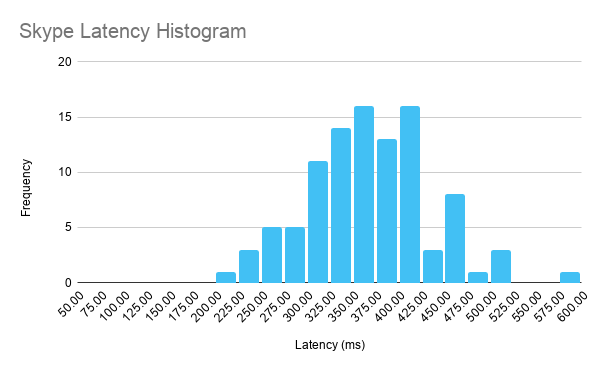
\includegraphics[width=\textwidth,height=3cm,keepaspectratio=true]{On5Skype}
    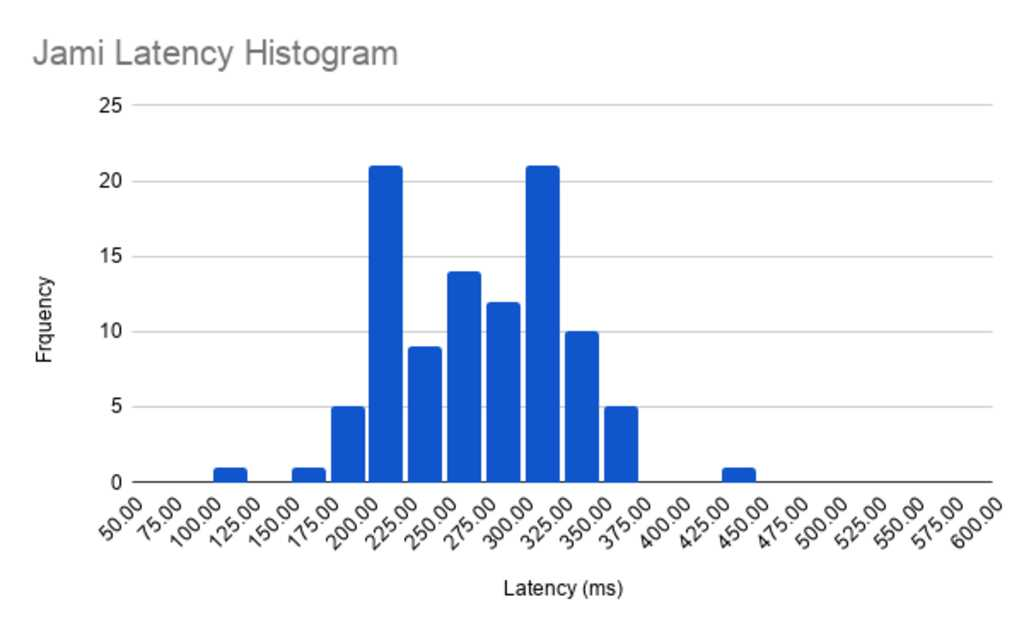
\includegraphics[width=\textwidth,height=3cm,keepaspectratio=true]{On5Jami}
    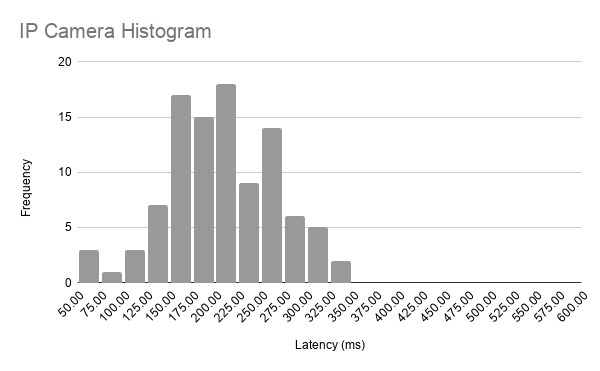
\includegraphics[width=\textwidth,height=3cm,keepaspectratio=true]{On5IPCam}
    \caption{
        Round-trip latency of the apps on a Samnsung On5.
    }
\end{figure}

\begin{figure}[!htb]
    \centering
    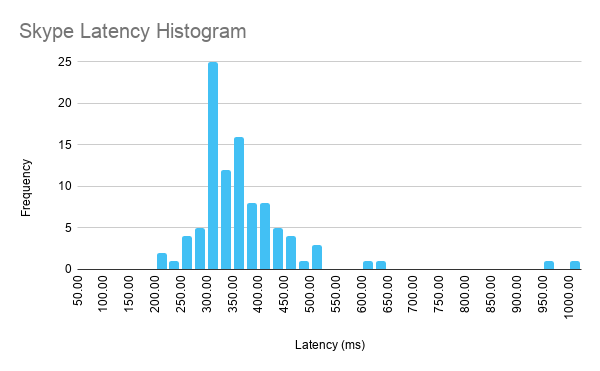
\includegraphics[width=\textwidth,height=3cm,keepaspectratio=true]{BladeSkype}
    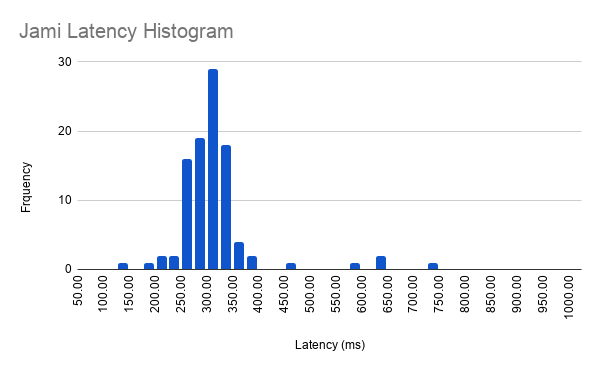
\includegraphics[width=\textwidth,height=3cm,keepaspectratio=true]{BladeJami}
    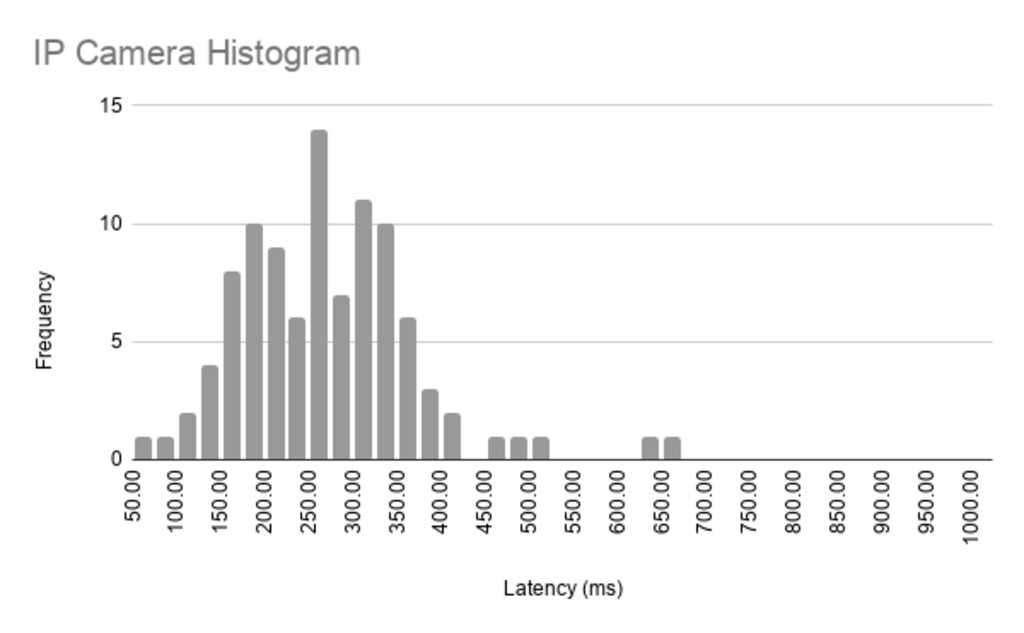
\includegraphics[width=\textwidth,height=3cm,keepaspectratio=true]{BladeIPCam}
    \caption{
        Round-trip latency of the apps on a ZTE Blade Max.
    }
\end{figure}

\begin{figure}[!htb]
    \centering
    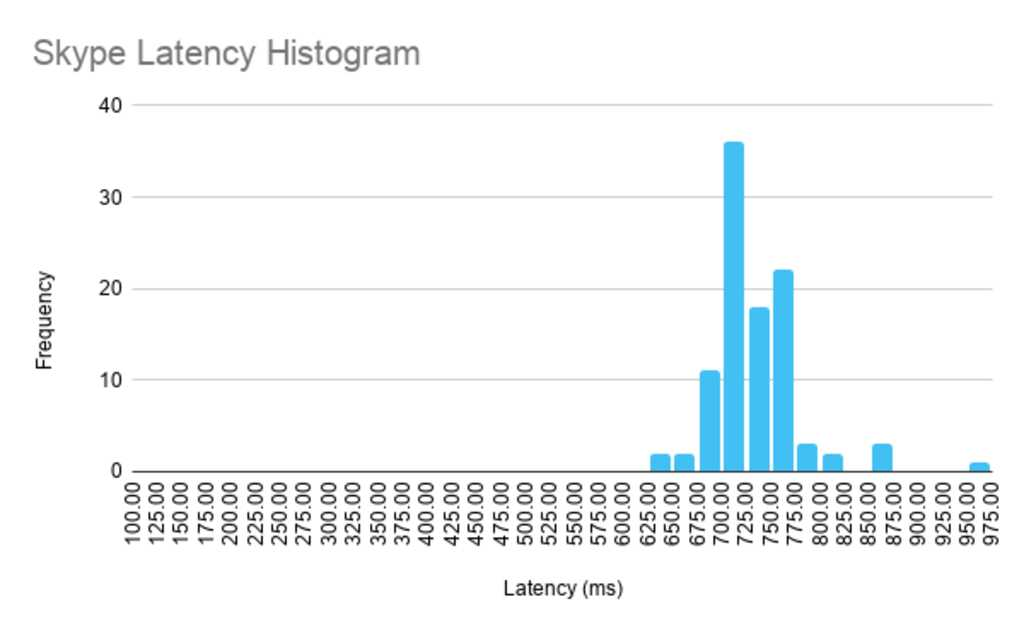
\includegraphics[width=\textwidth,height=3cm,keepaspectratio=true]{StyloSkype}
    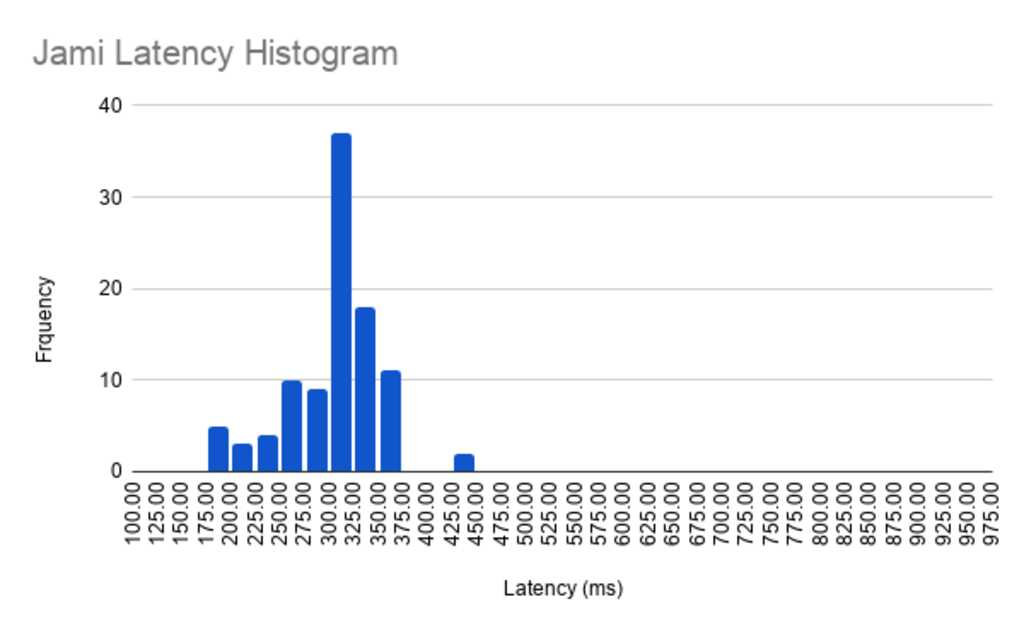
\includegraphics[width=\textwidth,height=3cm,keepaspectratio=true]{StyloJami}
    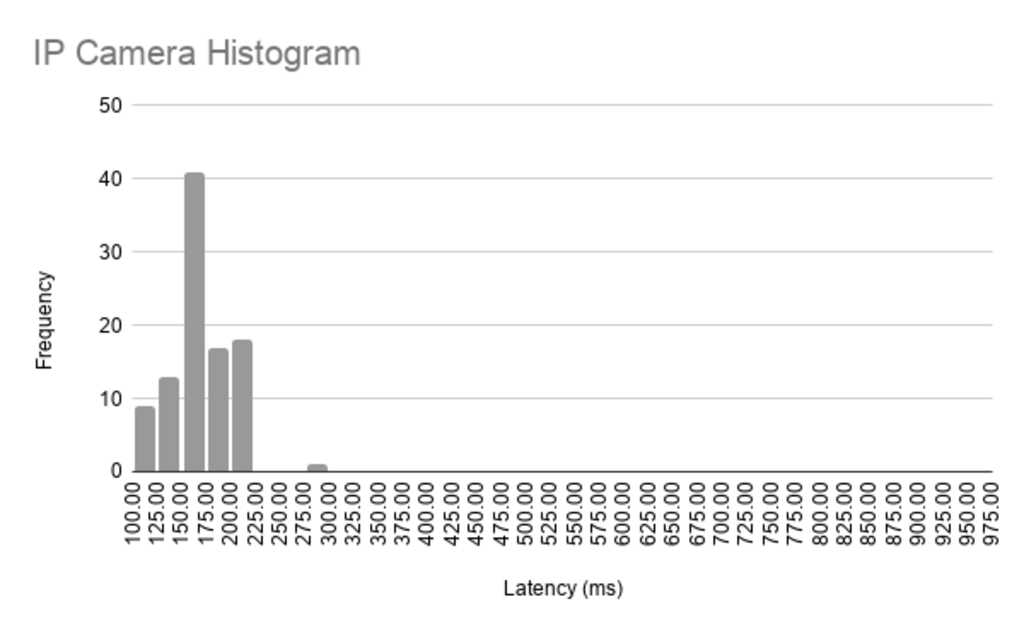
\includegraphics[width=\textwidth,height=3cm,keepaspectratio=true]{StyloIPCam}
    \caption{
        Round-trip latency of the apps on a LG Stylo 5.
    }
\end{figure}

\newpage
\subsection{Raspberry Pi Camera}
I wanted more quality. More speed. MORE POWER. Due to this, I got a Raspberry Pi 4 for Christmas, bought a camera module, and strived to push it to its limits.

\begin{figure}[!htb]
    \centering
    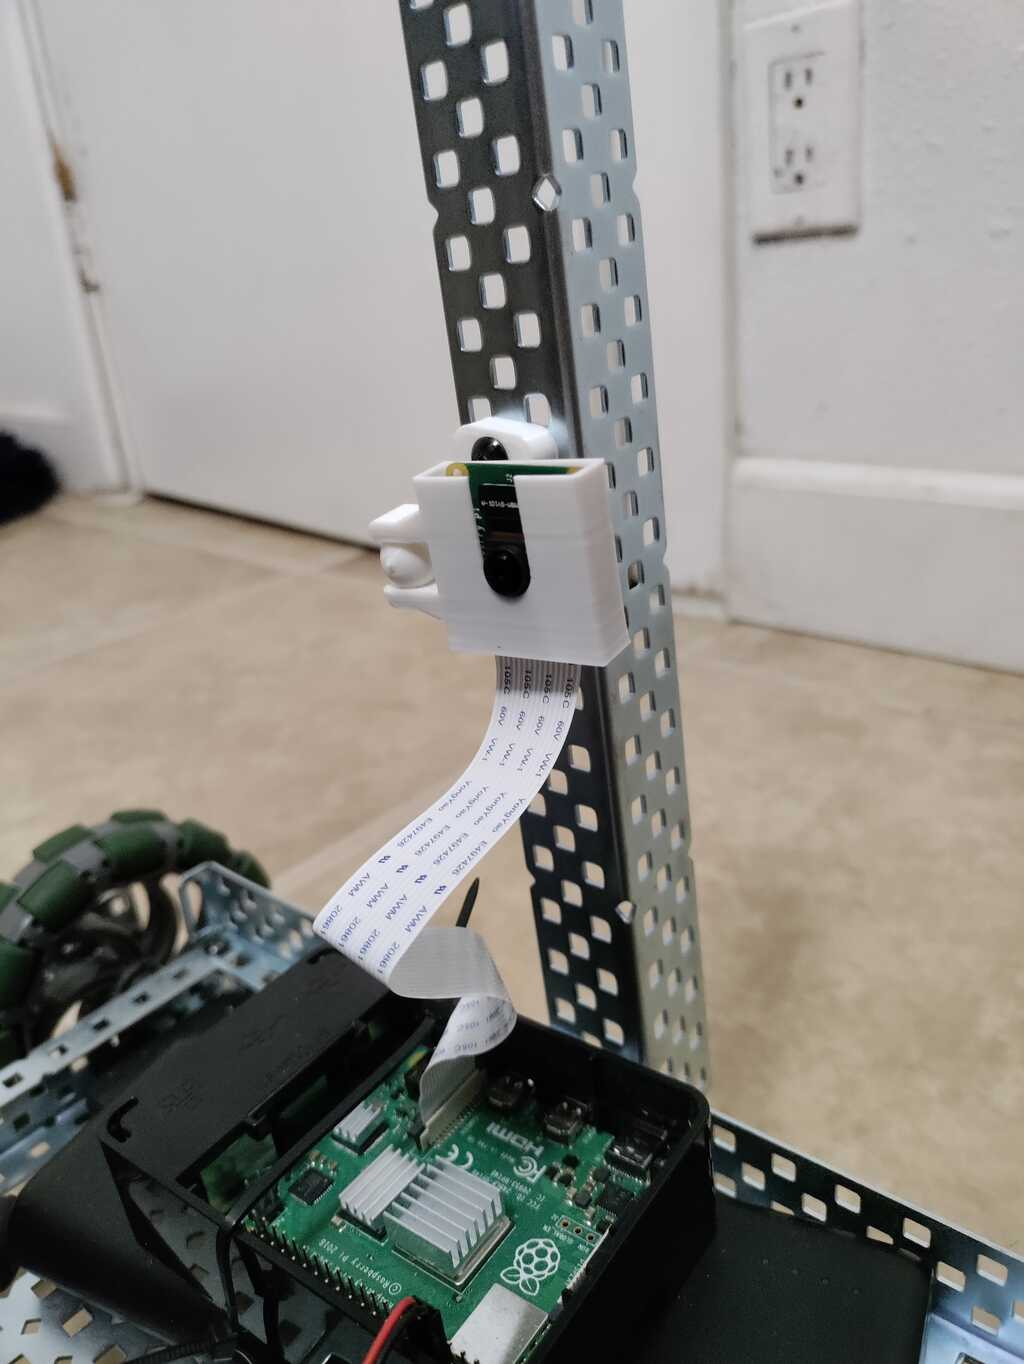
\includegraphics[width=\textwidth,height=6cm,keepaspectratio=true]{3DRaspCustom}
    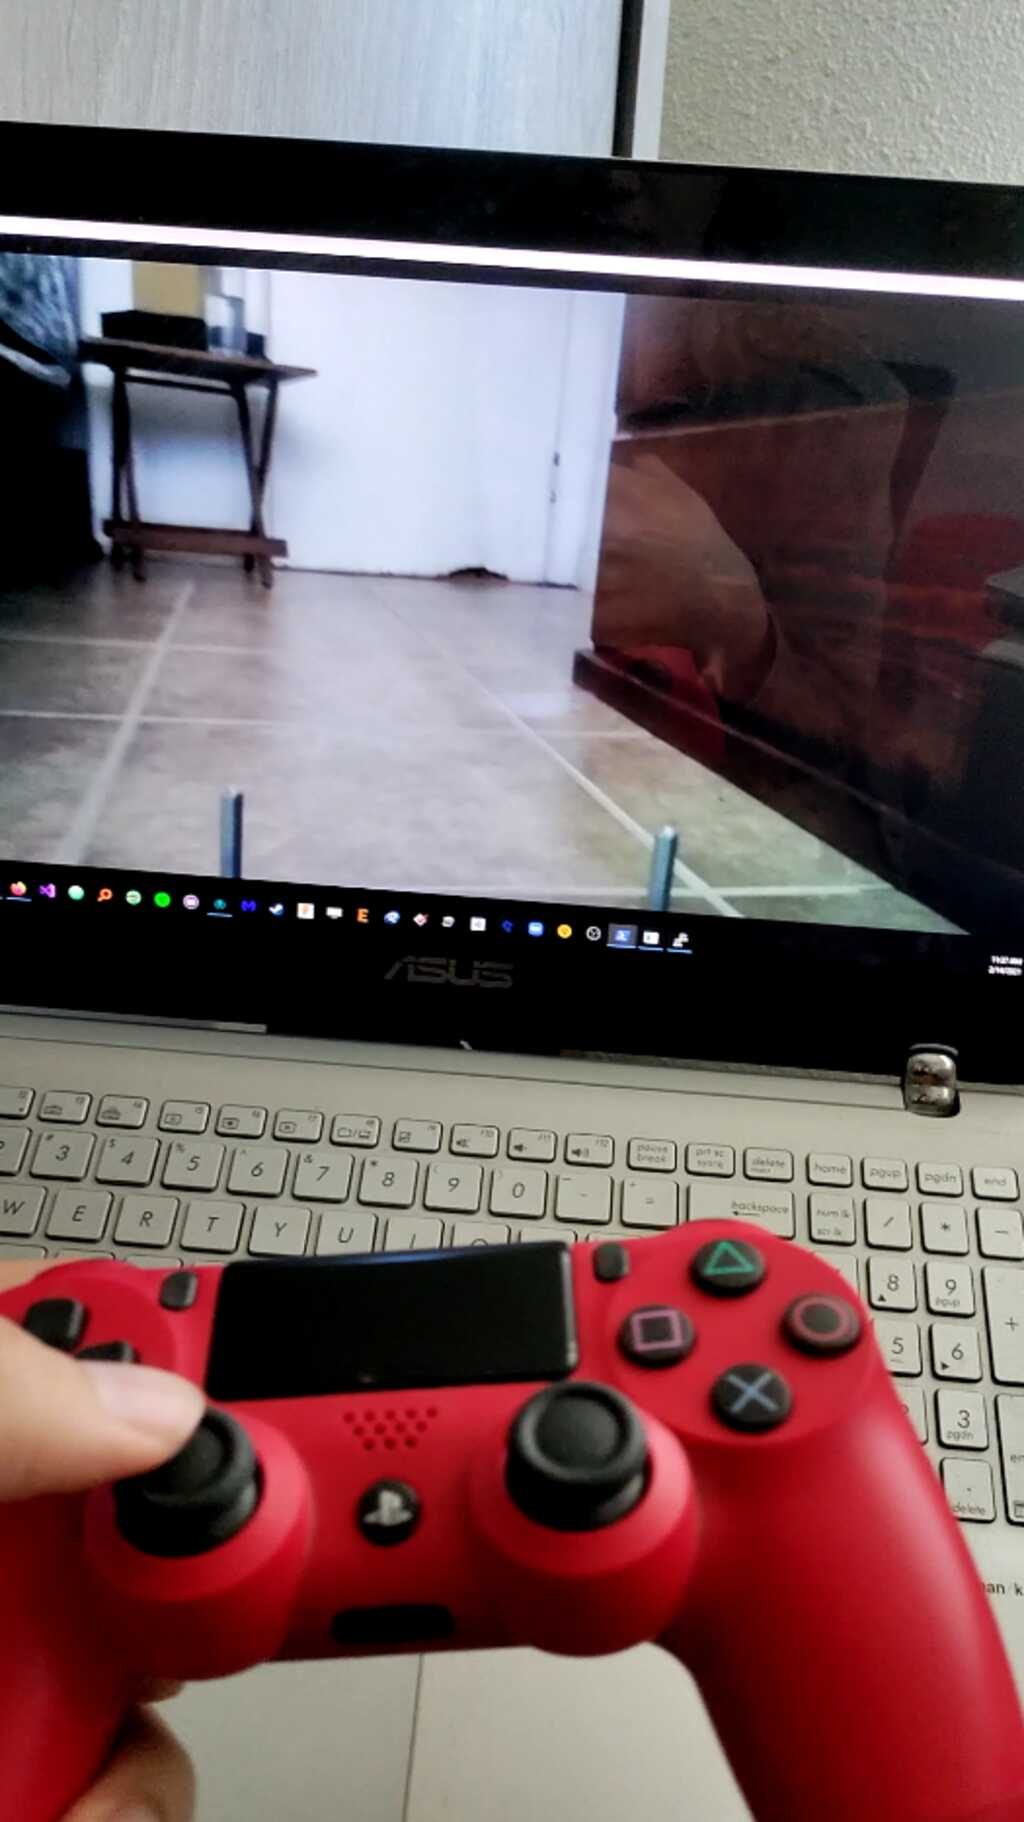
\includegraphics[width=\textwidth,height=6cm,keepaspectratio=true]{RemoteController}
    \caption{
        (Left) The finalized Raspberry Pi camera being mounted on the robot. (Right) live video feed of the camera being shown on the monitor.
    }
\end{figure}

Unfortunately, the solution to this problem was not easily solvable. The streaming scripts online focused primarily toward streaming over the internet, not a LAN. So I spent weeks finding and researching streaming libraries and the basics of networking until I derived two very special commands using a media-streaming library called gstreamer:

\begin{centering}

\textit{Raspberry Pi (Sender)}

\texttt{raspivid -n -t 0 -w \{width\} -h \{height\} -qp \{quality\} -fps \{fps\} --flush -b \{bitrate\} -o - | gst-launch-1.0 -e -vvvv fdsrc ! h264parse ! rtph264pay config-interval=1 pt=96 ! udpsink host=\{Linux Machine IP\} port=\{UDP port\}} \\[1cm]

\textit{Linux Machine (Receiver)}

\texttt{gst-launch-1.0 -e -v udpsrc address=\{Linux Machine IP\} port=\{UDP port\} ! application/x-rtp, payload=96 ! rtpjitterbuffer ! rtph264depay ! avdec\_h264 ! autovideosink sync=false}

\end{centering}

The sender command basically says this: feed the H.264-encoded video feed of the Raspberry Pi's camera (\texttt{raspivid}) into \texttt{gst-launch-1.0} (gstreamer) via the pipe operator \texttt{|} so that it gets sent to the receiver via a UCP connection. The receiving command simply decodes the data into a window.

While I am yet to offically collect data via a table, I can say, from experience, that this setup can stream 720p with less than 150 ms of latency at 30 fps; Something unheard of in weak Android phones. Due to this, I would consider using this camera as the main camera, with phone acting as backups / side cameras.
